\begin{figure}[h!]
  \begin{minipage}[c]{\textwidth}
    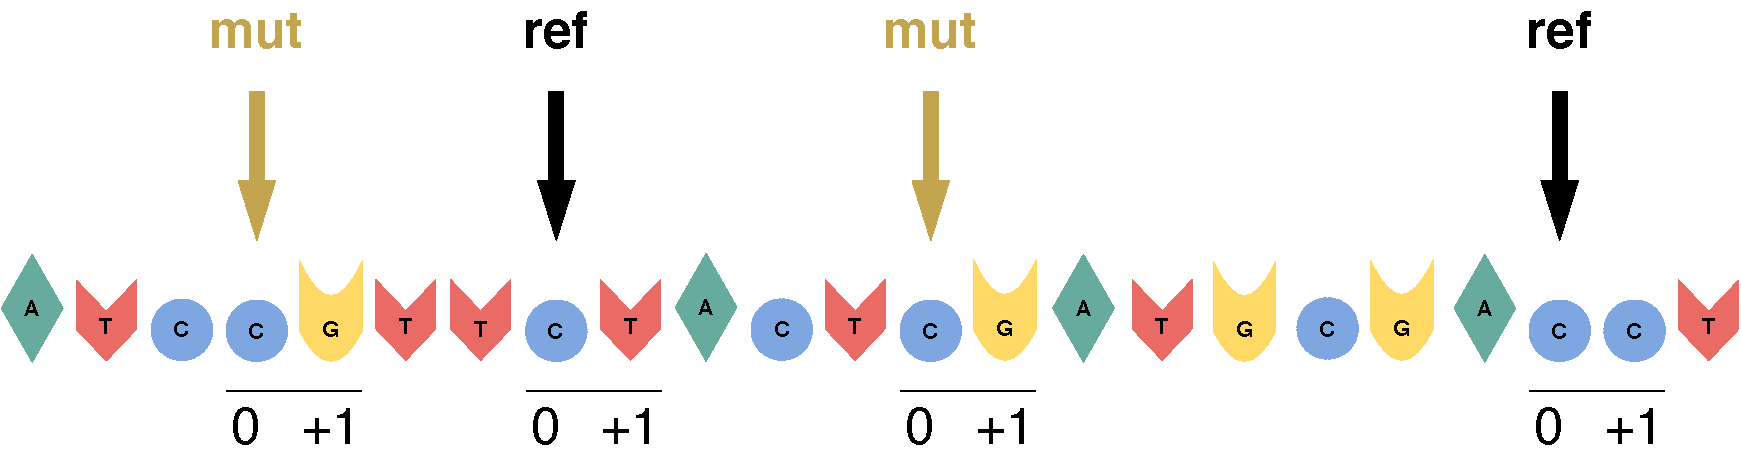
\includegraphics[width=\textwidth]{graphics/flank_demo.pdf}
  \end{minipage}\hfill
  \vspace{1cm}
  
  \begin{minipage}[c]{0.48\textwidth}
  \centering
    \begin{tabulary}{\columnwidth}{rRRRR}
    \toprule
        & \textbf{A} & \textbf{C} & \textbf{G} & \textbf{T}  \\
    \hline
        \textbf{mut} & 0 & 0 & 2 & 0  \\
        \textbf{ref} & 0 & 1 & 0 & 1  \\
    \bottomrule
    \end{tabulary}
  \end{minipage}\hfill
  \begin{minipage}[c]{0.48\textwidth}
    \begin{equation}
        \begin{aligned}
            H_o: \ln{count} =& \lambda_{status} + \lambda_{base} \\
            H_a: \ln{count} =& \lambda_{status} + \lambda_{base} + \lambda_{status:base}
        \end{aligned}
        \label{eq:nbr_demo}
    \end{equation}
  \end{minipage}
  \vspace{0.5cm}
  
  \begin{minipage}[c]{\textwidth}
    \caption{
    %   \textbf{Measuring information at position +1 of the C$\rightarrow$T mutation for Cancer A.} For each C$\rightarrow$T mutation, another C was randomly selected. I then counted the number of bases at flanking position +1 and presented them as a contingency table. In the figure, $\lambda_{base}$ is the indicator variable for the base at position +1, taking values \textbf{A, C, G, T}. $\lambda_{status}$ is the indicator variable for \textbf{mut} and \textbf{ref}; \textbf{mut} implies that the C is mutated into T, and \textbf{ref} implies the randomly selected base. Using the models in \ref{eq:nbr_demo}, I measured the relative entropy as described previously, the total $RE$ of all entries to the contingency table measures the amount of information at position +1. I did the same to all other positions within the 5-mer context and to all other mutations.
    } \label{fig:nbr_demo}
  \end{minipage}
\end{figure}
